
\section {Transkrip Percakapan Final Testing Web Service}
\begin{figure}[H]
	\centering
	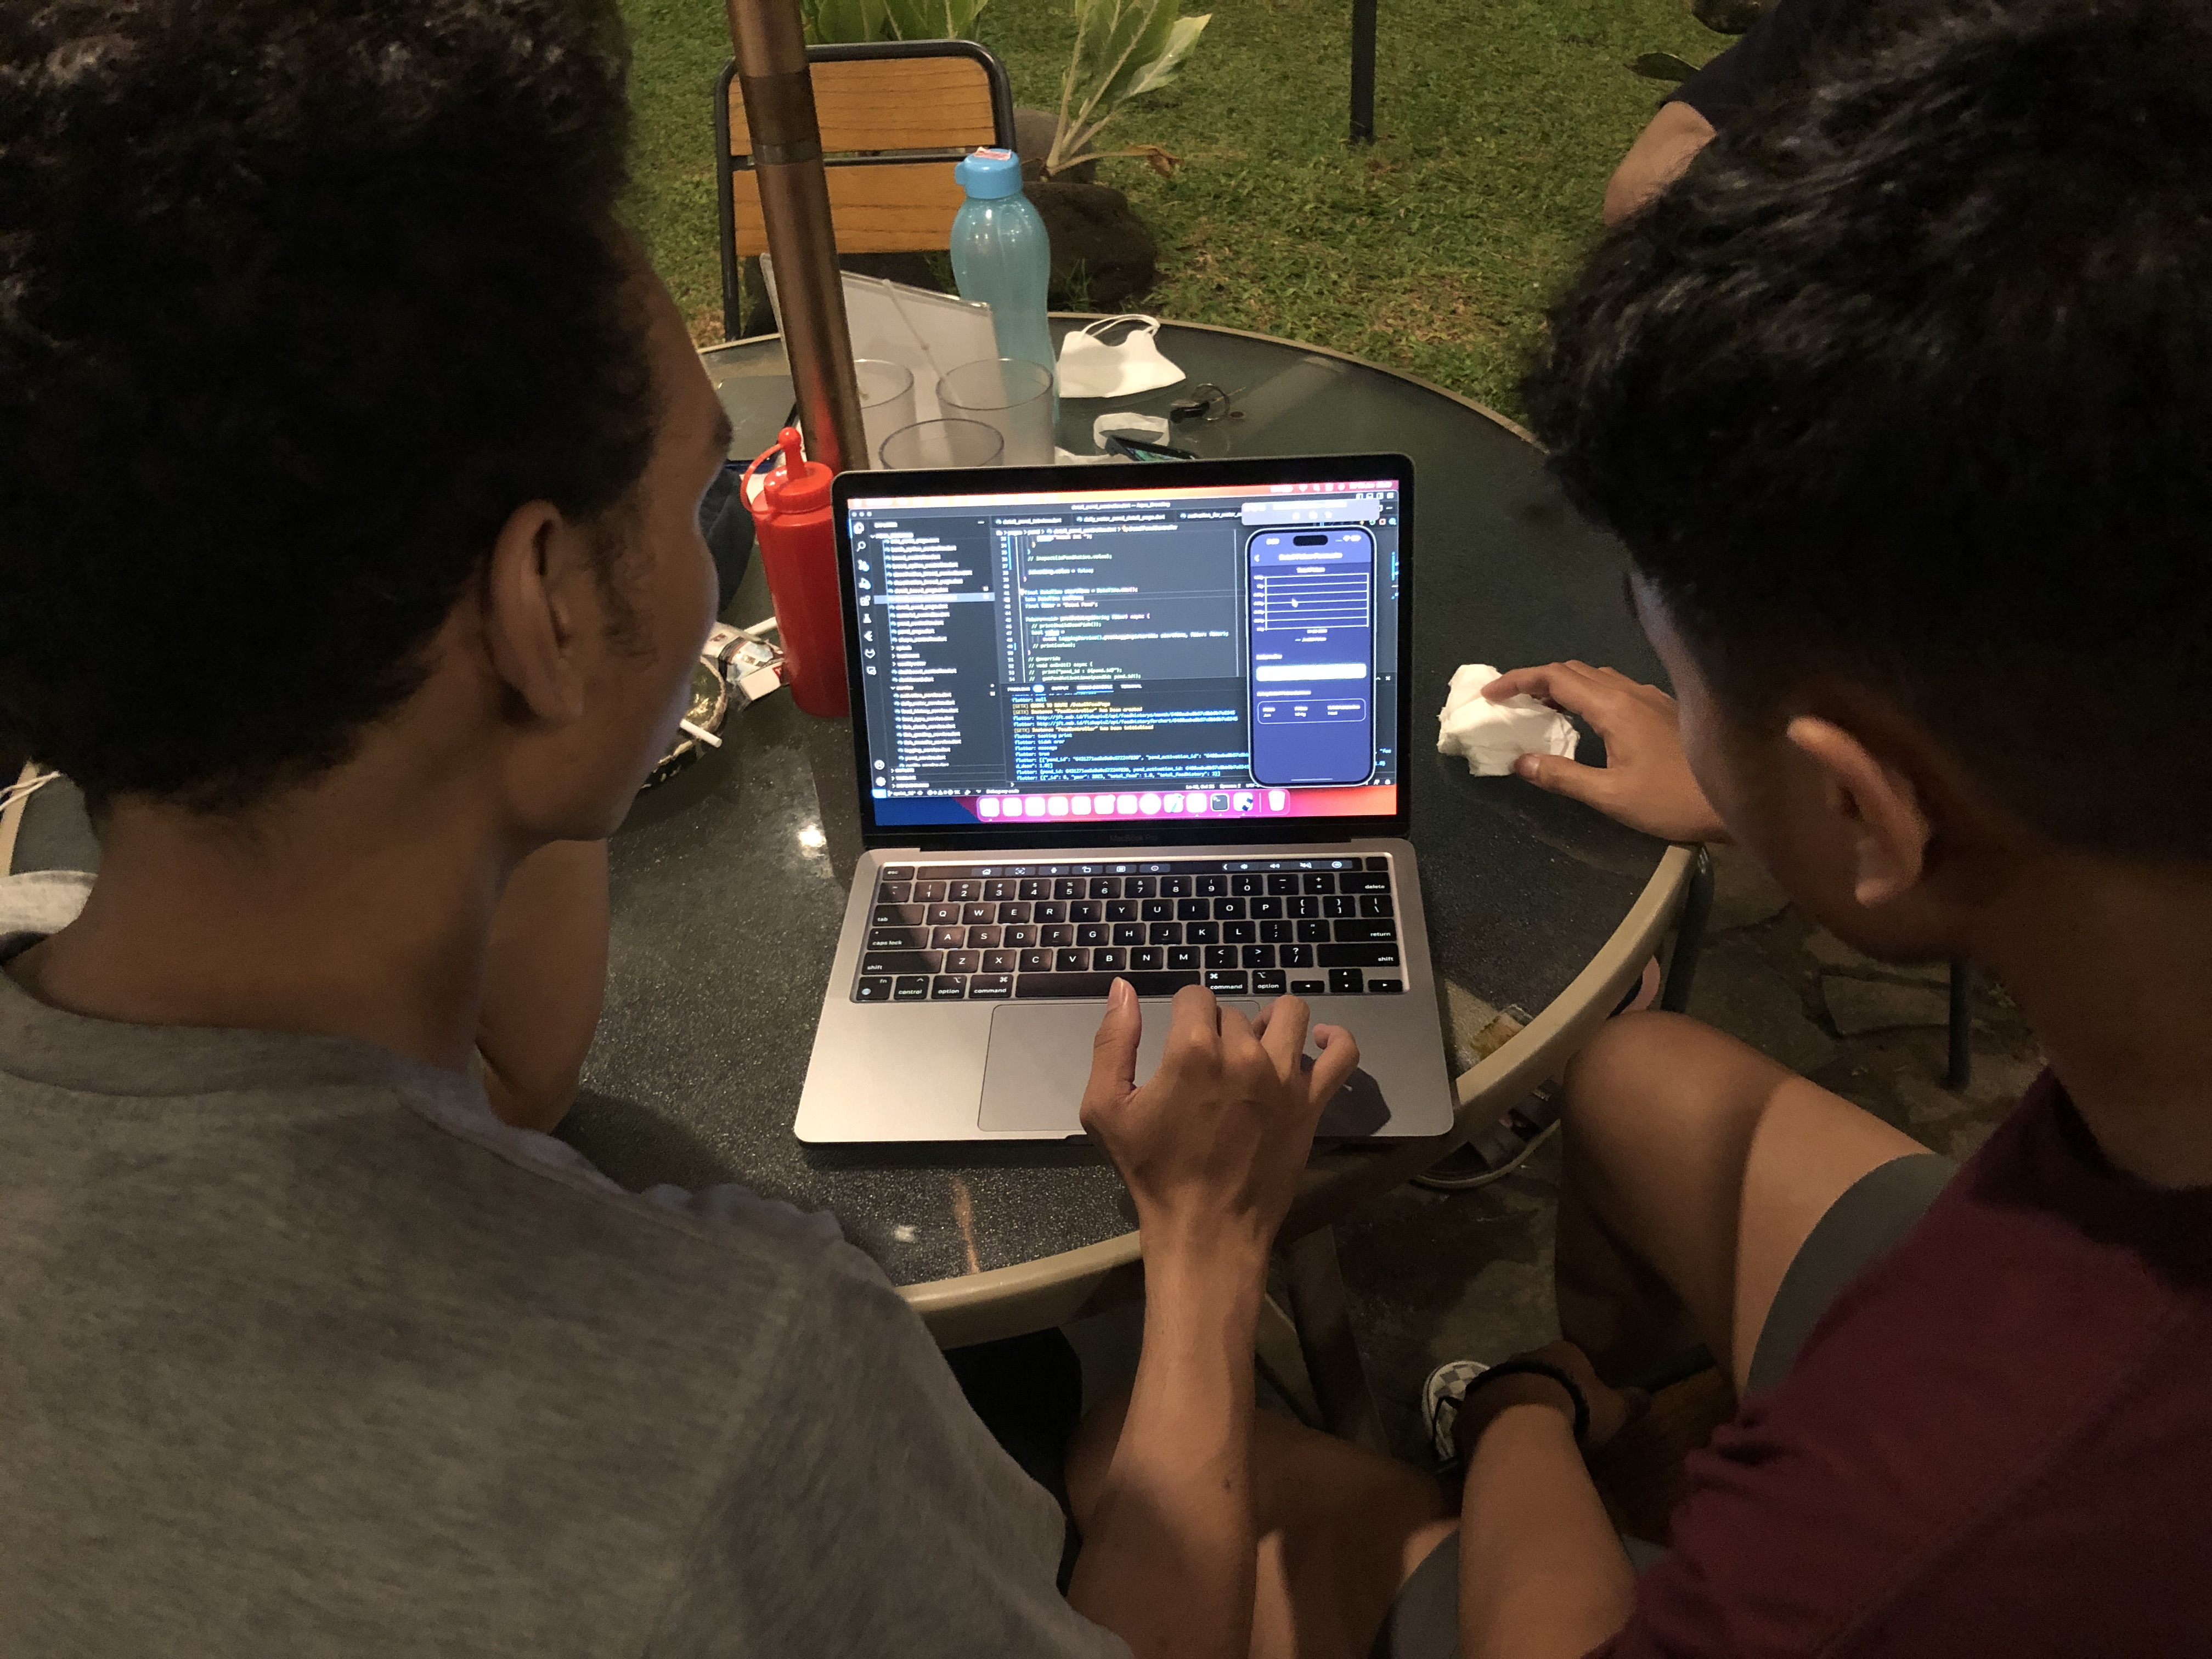
\includegraphics[width=1\textwidth]{gambar/img_testing_webservice.JPG}
	\caption{Dokumentasi UAT}
	\label{fig:img_uat}
\end{figure}
\begin{flushleft}
Hari: Jumat
\linebreak
Tanggal: 16 Juni 2023
\linebreak
Tempat: Upnoramal Raden Saleh
\linebreak
PL: Penulis
\linebreak
FD: Gian Chiesa (Frontend Developer)
\linebreak
\linebreak
PL: Assalamualikum Gi, Hari ini kita akan melakukan pengujian web service pada aplikasi
\linebreak
FD: Baik, untuk pengujian API saya melakukannya terhadap aplikasi aqua breeding yang telah dibuat menggunakan flutter dan dijalankan pada emulator andorid di mac os
\linebreak
PL: Oke bisa kita mulai pengujiannya
\linebreak
Dimulainya pengujian web service
\linebreak
PL: Baik, bagaimana hasil pengujian APInya?
\linebreak
FD: Secara keseluruhan API berhasil di implementasikan pada aplikasi, waktu respose API juga normal, dokumentasi pemakaian juga jelas, namun ada beberapa API yang baiknya disesuaikan responsenya karena kebutuhan User Experiance
\linebreak
PL: Apa contoh API yang harus disesuaikan?
\linebreak
FD: Seperti API Get list kolam, lebih baik setiap kolam ditambahkan keterangan jumlah ikan yang hidup, volume air kolam, dan keterangan jumlah ikan hidup / volume air kolam
PL: Baik Terima Kasih atas waktunya
\end{flushleft}